% ------------------------------------------------------------------------------
%						1 Introduction
% ------------------------------------------------------------------------------
\section{Introduction}
\label{sect:introduction}

This document contains basic information required to use ``Speed'', along with tips,
tricks, examples, and references to projects and papers that have used Speed.
User contributions of sample jobs and/or references are welcome.

\noindent \textbf{Note:}
On October 20, 2023, we completed the migration to SLURM from Grid Engine (UGE/AGE) as our job scheduler.
This manual has been updated to use SLURM's syntax and commands.
If you are a long-time GE user, refer to \xa{appdx:uge-to-slurm} for key highlights needed to
translate your GE jobs to SLURM as well as environment changes.
These changes are also elaborated throughout this document and our examples.

% 1.1 Citing US
% -------------------------------------------------------------
\subsection{Citing Us}
\label{sect:citing-speed-hpc}

If you wish to cite this work in your acknowledgements, you can use our general DOI found on our GitHub page
\url{https://dx.doi.org/10.5281/zenodo.5683642} or a specific version of the manual and scripts from that link individually.
You can also use the ``cite this repository'' feature of GitHub.

% 1.2 Resources
% -------------------------------------------------------------
\subsection{Resources}
\label{sect:resources}

\begin{itemize}
	\item
	Public GitHub page where the manual and sample job scripts are maintained at\\
	\url{https://github.com/NAG-DevOps/speed-hpc}
		\begin{itemize}
			\item Pull requests (PRs) are subject to review and are welcome:\\
			\url{https://github.com/NAG-DevOps/speed-hpc/pulls}
		\end{itemize}

	\item
	Speed Manual:
		\begin{itemize}
			\item PDF version of the manual:
			\url{https://github.com/NAG-DevOps/speed-hpc/blob/master/doc/speed-manual.pdf}
			\item HTML version of the manual:
			\url{https://nag-devops.github.io/speed-hpc/}
		\end{itemize}

	\item
	Concordia official page for ``Speed'' cluster, which includes access request instructions.
	\url{https://www.concordia.ca/ginacody/aits/speed.html}

	\item
	All Speed users are subscribed to the \texttt{hpc-ml} mailing list.
\end{itemize}

% 1.3 Team
% -------------------------------------------------------------
\subsection{Team}
\label{sect:speed-team}

Speed is supported by:
\begin{itemize}
	\item
	Serguei Mokhov, PhD, Manager, Networks, Security and HPC, AITS
	\item
	Gillian Roper, Senior Systems Administrator, HPC, AITS
	\item
	Carlos Alarcón Meza, Systems Administrator, HPC and Networking, AITS
	\item
	Farah Salhany, IT Instructional Specialist, AITS
\end{itemize}

We receive support from the rest of AITS teams, such as NAG, SAG, FIS, and DOG.

\url{https://www.concordia.ca/ginacody/aits.html}

% 1.4 What Speed Consists of
% -------------------------------------------------------------
\subsection{What Speed Consists of}
\label{sect:speed-arch}

\begin{itemize}
	\item Twenty four (24) 32-core compute nodes, each with 512~GB of memory and
	approximately 1~TB of local volatile-scratch disk space (pictured in \xf{fig:speed-front}).

	\item Twelve (12) NVIDIA Tesla P6 GPUs, with 16~GB of GPU memory (compatible with the
	CUDA, OpenGL, OpenCL, and Vulkan APIs).

	\item 4 VIDPRO nodes (ECE. Dr.~Amer), with 6 P6 cards, and 6 V100 cards (32GB), and
	256GB of RAM.

	\item 7 new SPEED2 servers with 256 CPU cores each 4x~A100 80~GB GPUs, partitioned
	into 4x~20GB MIGs each; larger local storage for TMPDIR (see \xf{fig:speed-architecture}).

	\item One AMD FirePro S7150 GPU, with 8~GB of memory (compatible with the
	Direct~X, OpenGL, OpenCL, and Vulkan APIs).

 	\item Salus compute node (CSSE CLAC, Drs.~Bergler and Kosseim), 56 cores and 728GB of RAM,
	see \xf{fig:speed-architecture}.

	\item Magic subcluster partition (ECE, Dr.~Khendek, 11 nodes, see \xf{fig:speed-architecture}).

	\item Nebular subcluster partition (CIISE, Drs.~Yan, Assi, Ghafouri, et al., Nebulae GPU node with 2x RTX 6000 Ada 48GB cards,
	Stellar compute node, and Matrix 177TB storage/compute node, see \xf{fig:speed-architecture}).
\end{itemize}

% Speed front image
\begin{figure}[htbp]
    \centering
    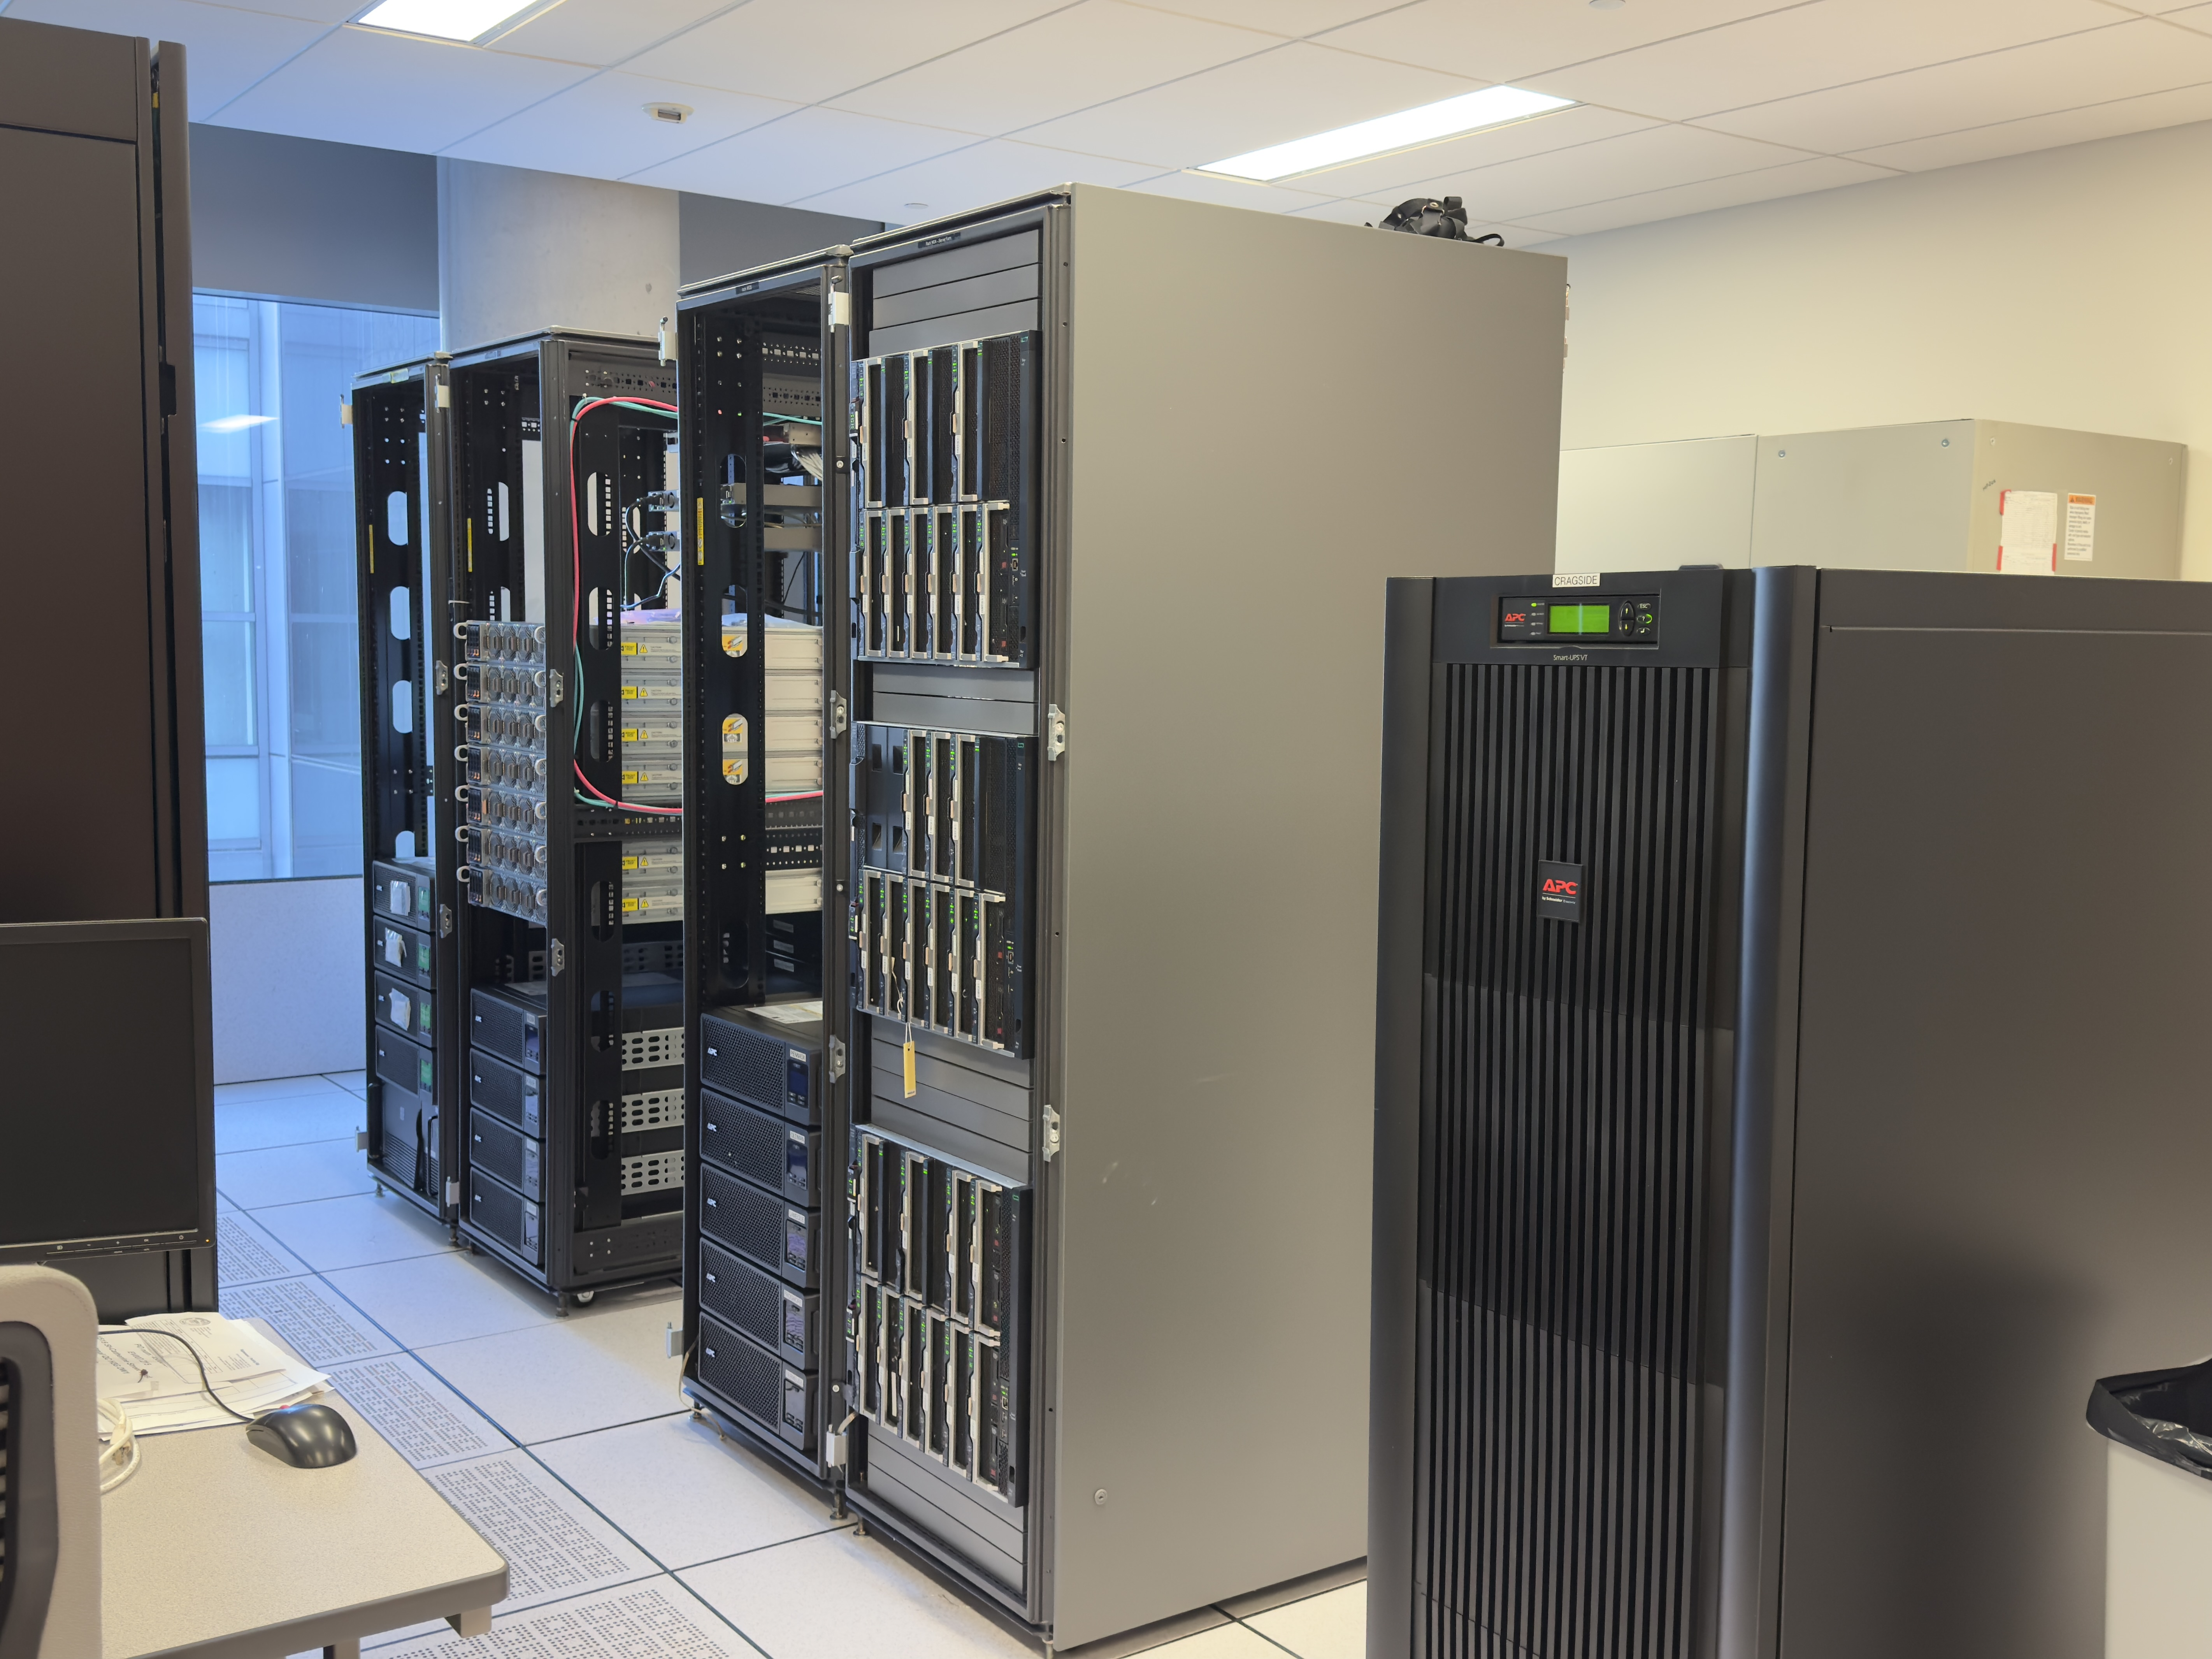
\includegraphics[width=0.9\columnwidth]{images/speed2.jpg}
    \caption{Speed Front}
    \label{fig:speed-front}
\end{figure}
\vspace{-1em}
% Speed back image
\begin{figure}[htbp]
    \centering
    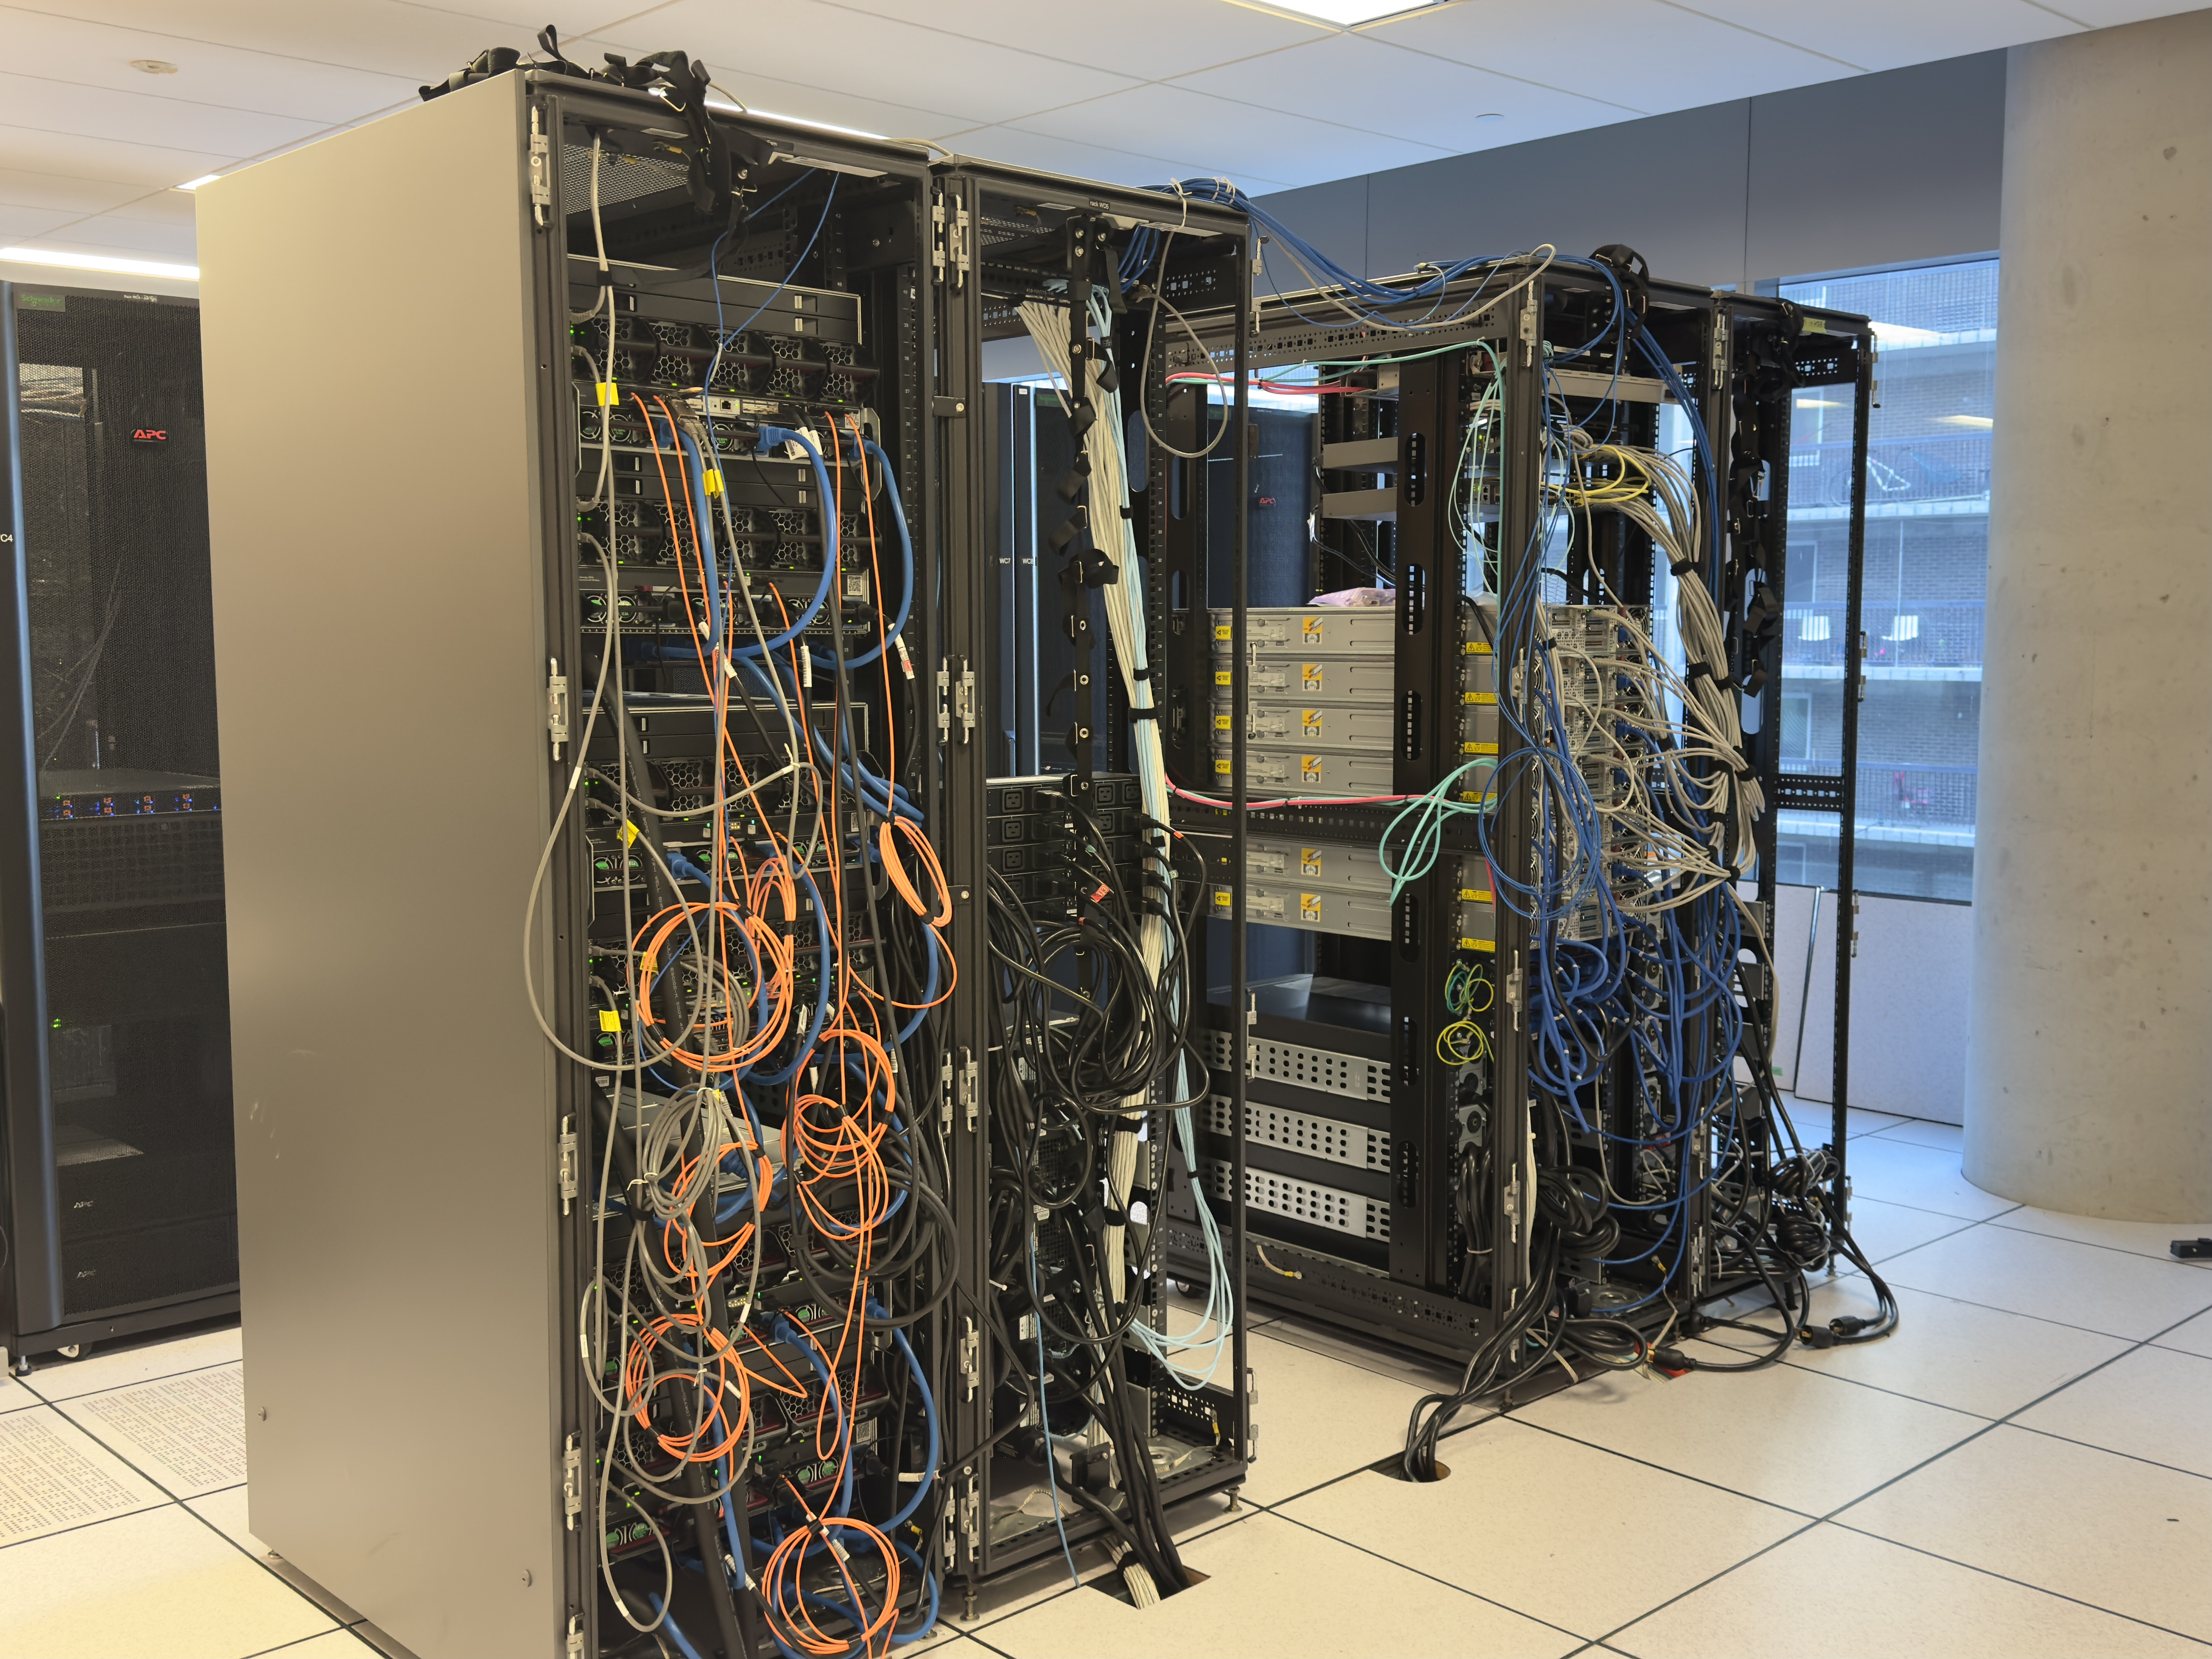
\includegraphics[width=0.9\columnwidth]{images/speed1.jpg}
    \caption{Speed Back}
    \label{fig:speed-back}
\end{figure}
\vspace{-1em}
% Speed architecture image
\begin{figure*}[htpb]
	\centering
	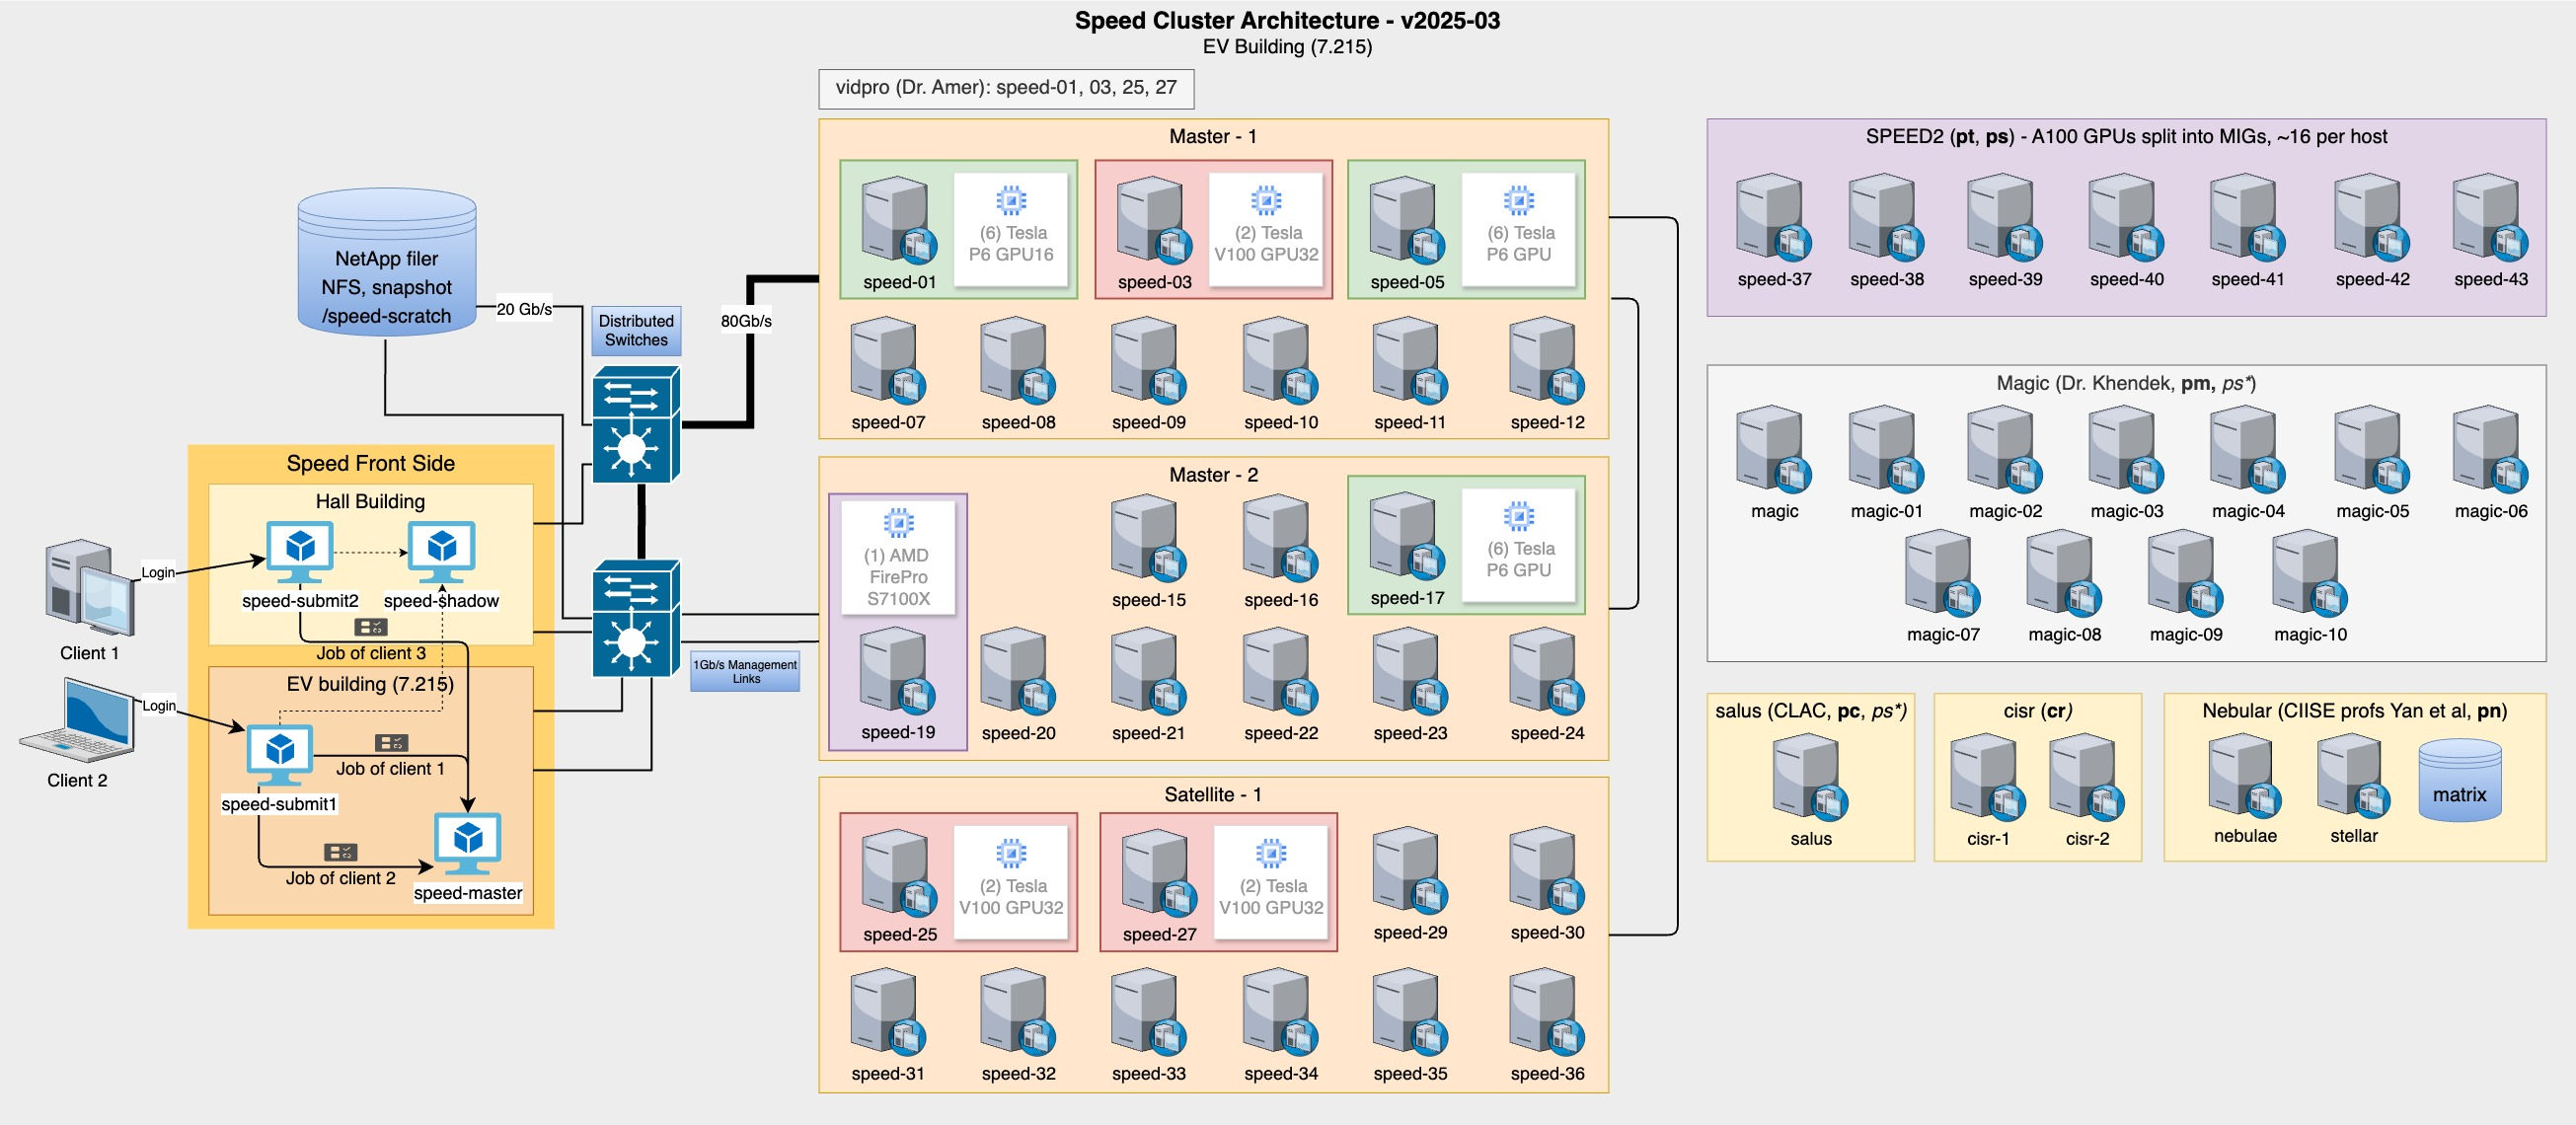
\includegraphics[width=\columnwidth]{images/SpeedArchitecture-March 2025.jpg}
	\caption{Speed Cluster Hardware Architecture}
	\label{fig:speed-architecture}
\end{figure*}
% Slurm architecture image
\begin{figure}[htpb]
	\centering
	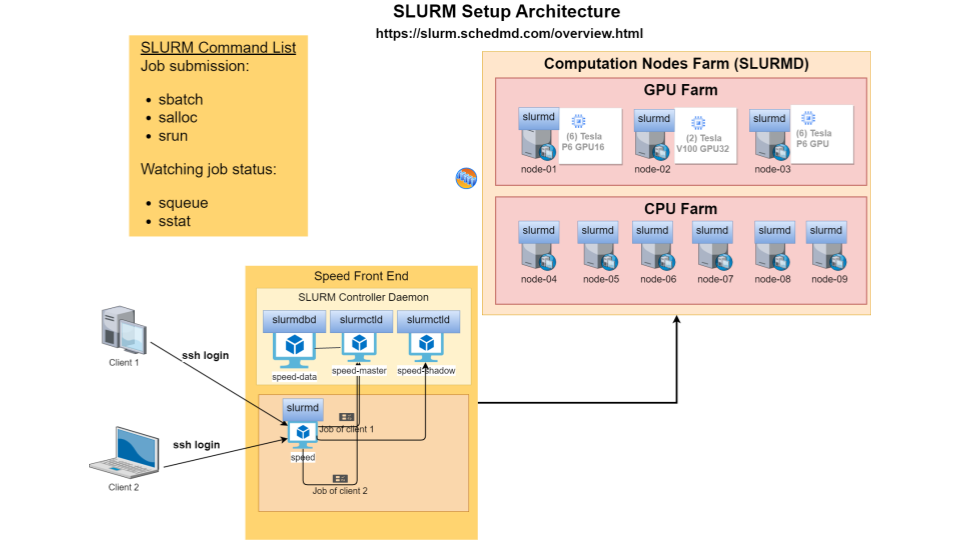
\includegraphics[width=\columnwidth]{images/slurm-arch}
	\caption{Speed SLURM Architecture}
	\label{fig:slurm-arch}
\end{figure}

% 1.5 What Speed Is Ideal For
% -------------------------------------------------------------
\subsection{What Speed Is Ideal For}
\label{sect:speed-is-for}

\begin{itemize}
	\item
	Design, develop, test, and run parallel, batch, and other algorithms and scripts with partial data sets.
	``Speed'' has been optimized for compute jobs that are multi-core aware,
	require a large memory space, or are iteration intensive.

	\item
	Prepare jobs for large clusters such as:
		\begin{itemize}
			\item Digital Research Alliance of Canada (Calcul Quebec and Compute Canada)
			\item Cloud platforms
		\end{itemize}
	\item
	Jobs that are too demanding for a desktop.
	\item
	Single-core batch jobs; multithreaded jobs typically up to 32 cores (i.e., a single machine).
	\item
	Multi-node multi-core jobs (MPI).
	\item
	Anything that can fit into a 500-GB memory space and a \textbf{speed scratch} space of approximately 10~TB. 
	\item
	CPU-based jobs.
	\item
	CUDA GPU jobs.
	\item
	Non-CUDA GPU jobs using OpenCL.
\end{itemize}

% 1.6 What Speed Is Not
% -------------------------------------------------------------
\subsection{What Speed Is Not}
\label{sect:speed-is-not}

\begin{itemize}
	\item Speed is not a web host and does not host websites.
	\item Speed is not meant for Continuous Integration (CI) automation deployments for Ansible or similar tools.
	\item Does not run Kubernetes or other container orchestration software.
	\item Does not run Docker. (\textbf{Note:} Speed does run Singularity and many Docker containers can be converted to
	Singularity containers with a single command. See \xs{sect:singularity-containers}.)
	\item Speed is not for jobs executed outside of the scheduler. (Jobs running outside of the scheduler will be killed and all data lost.)
\end{itemize}

% 1.7 Available Software
% -------------------------------------------------------------
\subsection{Available Software}
\label{sect:available-software}

There are a wide range of open-source and commercial software available and installed on ``Speed.''
This includes Abaqus~\cite{abaqus}, AllenNLP, Anaconda, ANSYS, Bazel,
COMSOL, CPLEX, CUDA, Eclipse, Fluent~\cite{fluent}, Gurobi, MATLAB~\cite{matlab,scholarpedia-matlab},
OMNeT++, OpenCV, OpenFOAM, OpenMPI, OpenPMIx, ParaView, PyTorch, QEMU, R, Rust, and Singularity among others.
Programming environments include various versions of Python, C++/Java compilers, TensorFlow, OpenGL, OpenISS, and {\marf}~\cite{marf}.

In particular, there are over 2200 programs available in \texttt{/encs/bin} and \texttt{/encs/pkg} under Scientific Linux 7 (EL7).
We are building an equivalent array of programs for the EL9 SPEED2 nodes. To see the packages available, run \texttt{ls -al /encs/pkg/} on \texttt{speed.encs}.
See a complete list in \xa{sect:software-list}.

\noindent\textbf{Note:} We do our best to accommodate custom software requests.
Python environments can use user-custom installs from within scratch directory.

% 1.8 Requesting Access
% ------------------------------------------------------------------------------
\subsection{Requesting Access}
\label{sect:access-requests}

After reviewing the ``What Speed is'' (\xs{sect:speed-is-for}) and
``What Speed is Not'' (\xs{sect:speed-is-not}), request access to the ``Speed''
cluster by emailing: \texttt{rt-ex-hpc AT encs.concordia.ca}.

\begin{itemize}
	\item GCS ENCS faculty and staff may request access directly.
	\item GCS students must include the following in their request message:
	\begin{itemize}
		\item GCS ENCS username
		\item Name and email (CC) of the approver -- either a supervisor, course instructor,
		or a department representative (e.g., in the case of undergraduate or M.Eng.\ students it
		can be the Chair, associate chair, a technical officer, or a department administrator) for approval.
		\item Written request from the approver for the GCS ENCS username to be granted access to ``Speed.''
	\end{itemize}
	\item Non-GCS students taking a GCS course will have their GCS ENCS account created automatically, but still need the course instructor's approval to use the service.
	\item Non-GCS faculty and students need to get a ``sponsor'' within GCS, so that a guest GCS ENCS account is created first. A sponsor can be any GCS Faculty member
	you collaborate with. Failing that, request the approval from our Dean's Office;
	via our Associate Deans Drs.~Eddie Hoi Ng or Emad Shihab.
	\item External entities collaborating with GCS Concordia researchers should also go through the Dean's Office for approvals.
\end{itemize}

For detailed instructions, refer to the Concordia
\href{https://www.concordia.ca/ginacody/aits/speed.html}{Computing (HPC) Facility: Speed} webpage.